\documentclass[border=10pt]{article}
% \usepackage{subfigure}
\usepackage{subcaption}
\usepackage{colortbl}
\usepackage{tikz}
\usetikzlibrary{decorations.pathmorphing, shapes}
\begin{document} 
\begin{figure}
  \centering
\begin{subfigure}{\textwidth}
  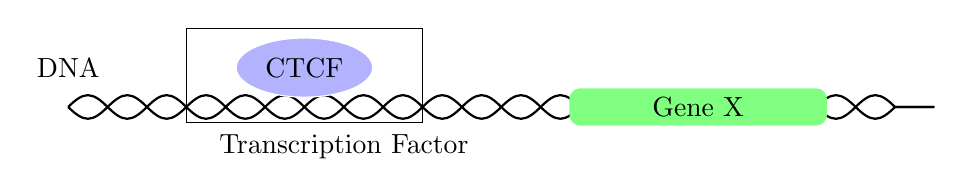
\begin{tikzpicture}[decoration={coil},
dna/.style={decorate, thick, decoration={aspect=0, segment length=1.0cm}},
protein/.style={ellipse, draw=white, minimum width=1cm, minimum height=1cm}]
 
%DNA
\draw[dna, decoration={amplitude=.15cm}] (.0,0) -- (11,0);
\draw[dna, decoration={amplitude=-.15cm}] (0,0) -- (11,0);
\node at (0,0.5) {DNA};
 
%Gene
 \node [rounded corners, fill=green!50, thick, inner xsep=30pt] at (8,0) (box){Gene X};
 \node [protein, minimum height=.75cm,fill=blue!30] at (3,0.5) {CTCF};
\node at (3.5, -0.5) {Transcription Factor};
\draw (1.5, -0.2) rectangle (4.5, 1); 
\end{tikzpicture}
\caption{Transcription factor binding to DNA, regulating the expression of Gene X}
\end{subfigure}
\begin{subfigure}{\textwidth}
  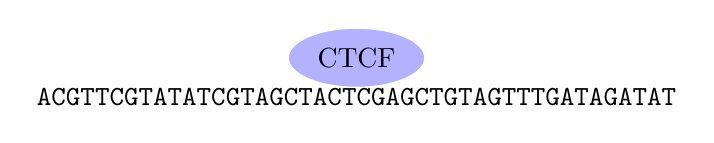
\begin{tikzpicture}[decoration={coil},
dna/.style={decorate, thick, decoration={aspect=0, segment length=1.0cm}},
protein/.style={ellipse, draw=white, minimum width=1cm, minimum height=1cm}]
\tikzstyle{seq}=[font=\ttfamily]
 
%DNA
\node[seq] at (3,0) {ACGTTCGTATATCGTAGCTACTCGAGCTGTAGTTTGATAGATAT};
%Gene
\node [protein, minimum height=.75cm,fill=blue!30] at (3,0.5) {CTCF};
\end{tikzpicture}
\end{subfigure}
\begin{subfigure}{\textwidth}
  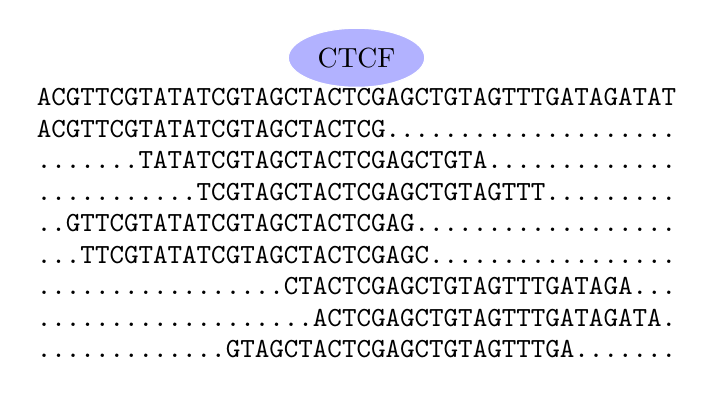
\begin{tikzpicture}[decoration={coil},
dna/.style={decorate, thick, decoration={aspect=0, segment length=1.0cm}},
protein/.style={ellipse, draw=white, minimum width=1cm, minimum height=1cm}]
seq/.style={font=\ttfamily}
\tikzstyle{seq}=[font=\ttfamily]
\def\fy{0.4}
% DNA
\node[seq] at (3, 0*\fy) {ACGTTCGTATATCGTAGCTACTCGAGCTGTAGTTTGATAGATAT};
\node[seq] at (3,-1*\fy) {ACGTTCGTATATCGTAGCTACTCG....................};
\node[seq] at (3,-2*\fy) {.......TATATCGTAGCTACTCGAGCTGTA.............};
\node[seq] at (3,-3*\fy) {...........TCGTAGCTACTCGAGCTGTAGTTT.........};
\node[seq] at (3,-4*\fy) {..GTTCGTATATCGTAGCTACTCGAG..................};
\node[seq] at (3,-5*\fy) {...TTCGTATATCGTAGCTACTCGAGC.................};
\node[seq] at (3,-6*\fy) {.................CTACTCGAGCTGTAGTTTGATAGA...};
\node[seq] at (3,-7*\fy) {...................ACTCGAGCTGTAGTTTGATAGATA.};
\node[seq] at (3,-8*\fy) {.............GTAGCTACTCGAGCTGTAGTTTGA.......};
%Gene
\node [protein, minimum height=.75cm,fill=blue!30] at (3,0.5) {CTCF};
%0, 7, 11, 2, 3, 17, 19, 13
% 0, 2, 3, 7, 11, 13, 17, 19
\end{tikzpicture}
\caption{DNA Fragments obtained form ChIP}
\end{subfigure}
\begin{subfigure}{\textwidth}
  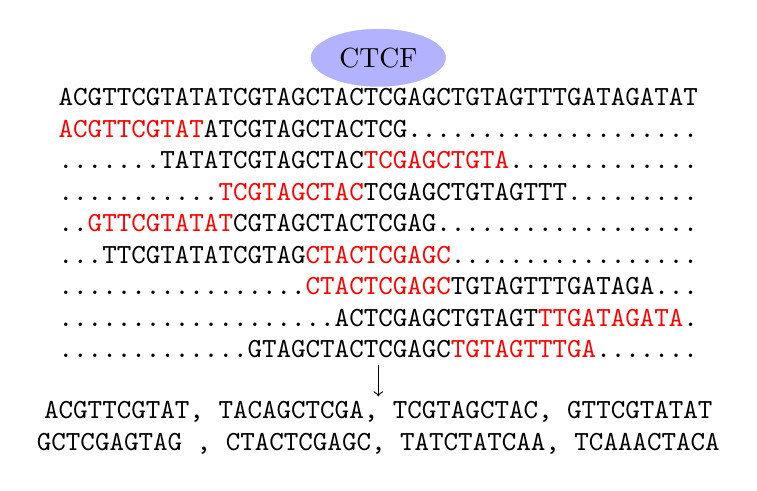
\begin{tikzpicture}[decoration={coil},
dna/.style={decorate, thick, decoration={aspect=0, segment length=1.0cm}},
protein/.style={ellipse, draw=white, minimum width=1cm, minimum height=1cm}]
seq/.style={font=\ttfamily}
\tikzstyle{seq}=[font=\ttfamily]
\def\fy{0.4}
\node [protein, minimum height=.75cm,fill=blue!30] at (3,0.5) {CTCF};

% DNA
\node[seq] at (3, 0*\fy) {ACGTTCGTATATCGTAGCTACTCGAGCTGTAGTTTGATAGATAT};
\node[seq] at (3,-1*\fy) {\textcolor{red}{ACGTTCGTAT}ATCGTAGCTACTCG....................};
\node[seq] at (3,-2*\fy) {.......TATATCGTAGCTAC\textcolor{red}{TCGAGCTGTA}.............};
\node[seq] at (3,-3*\fy) {...........\textcolor{red}{TCGTAGCTAC}TCGAGCTGTAGTTT.........};
\node[seq] at (3,-4*\fy) {..\textcolor{red}{GTTCGTATAT}CGTAGCTACTCGAG..................};
\node[seq] at (3,-5*\fy) {...TTCGTATATCGTAG\textcolor{red}{CTACTCGAGC}.................};
\node[seq] at (3,-6*\fy) {.................\textcolor{red}{CTACTCGAGC}TGTAGTTTGATAGA...};
\node[seq] at (3,-7*\fy) {...................ACTCGAGCTGTAGT\textcolor{red}{TTGATAGATA}.};
\node[seq] at (3,-8*\fy) {.............GTAGCTACTCGAGC\textcolor{red}{TGTAGTTTGA}.......};
% Gene
\draw[->] (3, -8.5*\fy) -- (3, -9.5*\fy);
\node[seq] at (3, -10*\fy) {ACGTTCGTAT, TACAGCTCGA, TCGTAGCTAC, GTTCGTATAT};
\node[seq] at (3, -11*\fy) {GCTCGAGTAG , CTACTCGAGC, TATCTATCAA, TCAAACTACA};
\end{tikzpicture}
\caption{One end of each fragment is sequenced}
\end{subfigure}
\begin{subfigure}{\textwidth}
  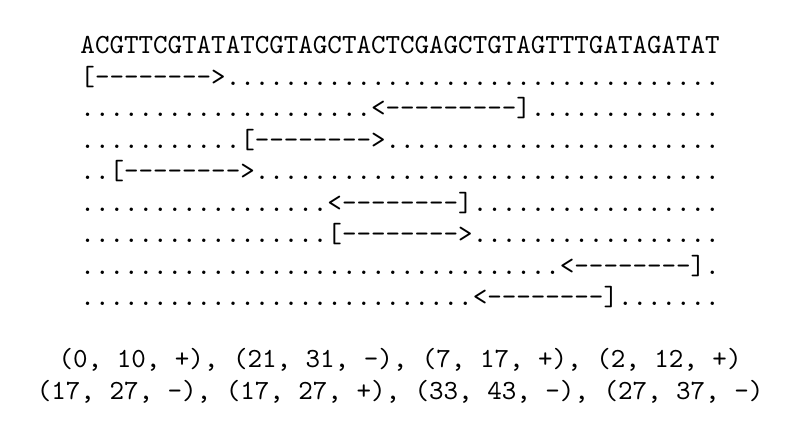
\begin{tikzpicture}[decoration={coil},
dna/.style={decorate, thick, decoration={aspect=0, segment length=1.0cm}},
protein/.style={ellipse, draw=white, minimum width=1cm, minimum height=1cm}]
\tikzstyle{seq}=[font=\ttfamily]
 \def\fy{0.4}
%DNA
\node[seq] at (3,0)      {ACGTTCGTATATCGTAGCTACTCGAGCTGTAGTTTGATAGATAT};
\node[seq] at (3,-1*\fy) {[-------->..................................};
\node[seq] at (3,-2*\fy) {....................<---------].............};
\node[seq] at (3,-3*\fy) {...........[-------->.......................};
\node[seq] at (3,-4*\fy) {..[-------->................................};
\node[seq] at (3,-5*\fy) {.................<--------].................};
\node[seq] at (3,-6*\fy) {.................[-------->.................};
\node[seq] at (3,-7*\fy) {.................................<--------].};
\node[seq] at (3,-8*\fy) {...........................<--------].......};
% 0, 7, 11, 2,
% 3, 17, 19, 13
\node[seq] at (3, -10*\fy) {(0, 10, +), (21, 31, -), (7, 17, +), (2, 12, +)};
\node[seq] at (3, -11*\fy) {(17, 27, -), (17, 27, +), (33, 43, -), (27, 37, -)};
\end{tikzpicture}
\caption{Sequenced reads mapped to the reference genome}
\end{subfigure}
\end{figure}
\begin{tabular}{| r | r | r | r |}
  \hline
  Interval & Extended & Sorted\\
  \hline
  (0, 10, +)  & (0, 24)  & (0, 24) \\
  (21, 31, -) & (7, 31)  & (2, 26) \\
  (7, 17, +)  & (7, 31)  & (3, 27) \\
  (2, 12, +)  & (2, 26)  & (7, 31) \\
  (17, 27, -) & (3, 27)  & (7, 31) \\
  (17, 27, +) & (17, 41) & (13, 37)\\
  (33, 43, -) & (19, 43) & (17, 41)\\
  (27, 37, -) & (13, 37) & (19, 43)\\
  \hline
              & $O(n)$   & $O(n \log n)$\\
  \hline
\end{tabular}
\begin{tabular}{|r|r|r|r|r|}
  \hline
  Index & Diff & Value & P-value & Peak \\
  \hline
  0  & 1  & 1 & 0.93 & 0 \\
  2  & 1  & 2 & 0.81 & 0 \\
  3  & 1  & 3 & 0.63 & 0 \\
  7  & 2  & 5 & 0.27 & 0 \\
  13 & 1  & 6 & 0.15 & 0 \\
  17 & 1  & 7 & 0.08 & 0 \\
  19 & 1  & 8 & 0.03 & 1 \\
  24 & -1 & 7 & 0.08 & 0 \\
  26 & -1 & 6 & 0.15 & 0 \\
  27 & -1 & 5 & 0.27 & 0 \\
  31 & -2 & 3 & 0.63 & 0 \\
  37 & -1 & 2 & 0.81 & 0 \\
  41 & -1 & 1 & 0.93 & 0 \\
  43 & -1 & 0 & 0.99 & 0 \\
  \hline
\end{tabular}
yielding the interval $\left[19, 24\right)$ as the only peak.

In a real experiment, more intervals would be yielded which would be affected by noise in the experiment. 
In order to reduce the effect of noise, two postprocessing steps are performed. First, small gaps between intervals are removed, then small peaks are removed:

\begin{tabular}{| r | r | r | r |}
  \hline
  Interval & Small Gaps Filled & Small Peaks Removed \\
  \hline
  (121, 125) & \textcolor{red}{(121, 125)} &  \\
  (142, \textcolor{red}{147)} & (142,      & (142, \\
  \textcolor{red}{(151, } 166) & 166)    & 166)\\
  (172, 200) & (172, 200) & (172, 200) \\
  \hline
\end{tabular}
\clearpage
\begin{table}
\begin{tabular}{|>{\columncolor[gray]{0.8}}r |r|r|r|r|r|r|r|r|r|r|r|r|r|r|r|>{\columncolor[gray]{0.8}}r|}
\$ & A & C & G & T & T & A & C & G & G & T & A & C & C & G & T & A \\
A & \$ & A & C & G & T & T & A & C & G & G & T & A & C & C & G & T \\
A & C & C & G & T & A & \$ & A & C & G & T & T & A & C & G & G & T \\
A & C & G & G & T & A & C & C & G & T & A & \$ & A & C & G & T & T \\
A & C & G & T & T & A & C & G & G & T & A & C & C & G & T & A & \$ \\
C & C & G & T & A & \$ & A & C & G & T & T & A & C & G & G & T & A \\
C & G & G & T & A & C & C & G & T & A & \$ & A & C & G & T & T & A \\
C & G & T & A & \$ & A & C & G & T & T & A & C & G & G & T & A & C \\
C & G & T & T & A & C & G & G & T & A & C & C & G & T & A & \$ & A \\
G & G & T & A & C & C & G & T & A & \$ & A & C & G & T & T & A & C \\
G & T & A & \$ & A & C & G & T & T & A & C & G & G & T & A & C & C \\
G & T & A & C & C & G & T & A & \$ & A & C & G & T & T & A & C & G \\
G & T & T & A & C & G & G & T & A & C & C & G & T & A & \$ & A & C \\
T & A & \$ & A & C & G & T & T & A & C & G & G & T & A & C & C & G \\
T & A & C & C & G & T & A & \$ & A & C & G & T & T & A & C & G & G \\
T & A & C & G & G & T & A & C & C & G & T & A & \$ & A & C & G & T \\
T & T & A & C & G & G & T & A & C & C & G & T & A & \$ & A & C & G \\
\end{tabular}
\end{table}
\begin{table}
\begin{tabular}{|r|>{\columncolor[gray]{0.8}}r|r|r|r|r|r|r|r|r|r|r|r|r|r|r|r|>{\columncolor[gray]{0.8}}r|}
16 & \$ & A & C & G & T & T & A & C & G & G & T & A & C & C & G & T & A\\ 
15 & A & \$ & A & C & G & T & T & A & C & G & G & T & A & C & C & G & T\\ 
10 & A & C & C & G & T & A & \$ & A & C & G & T & T & A & C & G & G & T\\ 
5 & A & C & G & G & T & A & C & C & G & T & A & \$ & A & C & G & T & T\\ 
0 & A & C & G & T & T & A & C & G & G & T & A & C & C & G & T & A & \$\\ 
11 & C & C & G & T & A & \$ & A & C & G & T & T & A & C & G & G & T & A\\ 
6 & C & G & G & T & A & C & C & G & T & A & \$ & A & C & G & T & T & A\\ 
12 & C & G & T & A & \$ & A & C & G & T & T & A & C & G & G & T & A & C\\ 
1 & C & G & T & T & A & C & G & G & T & A & C & C & G & T & A & \$ & A\\ 
7 & G & G & T & A & C & C & G & T & A & \$ & A & C & G & T & T & A & C\\ 
13 & G & T & A & \$ & A & C & G & T & T & A & C & G & G & T & A & C & C\\ 
8 & G & T & A & C & C & G & T & A & \$ & A & C & G & T & T & A & C & G\\ 
2 & G & T & T & A & C & G & G & T & A & C & C & G & T & A & \$ & A & C\\ 
14 & T & A & \$ & A & C & G & T & T & A & C & G & G & T & A & C & C & G\\ 
9 & T & A & C & C & G & T & A & \$ & A & C & G & T & T & A & C & G & G\\ 
4 & T & A & C & G & G & T & A & C & C & G & T & A & \$ & A & C & G & T\\ 
3 & T & T & A & C & G & G & T & A & C & C & G & T & A & \$ & A & C & G
\end{tabular}\end{table}

\end{document}

%%% Local Variables:
%%% mode: latex
%%% TeX-master: t
%%% End:
